\begin{pastexam}[label={px:ncku-108-ee-ds-07}]{成大電機所 108 學年度 問答題第 6 題}
（問答）

Draw a suffix trie for the following sequence, S=acbabbabb. Locate the position where ``abb''
occurs. (10 points)
\end{pastexam}

\begin{pastsoln}
後綴 trie 是把 $S$ 的所有後綴插進同一棵 trie（資結書第~11.5.5~節）。 照資結書的做法在結尾加一個不在
字母表裡的符號 \texttt{\$}，讓每個後綴都停在自己的葉節點（否則像 \texttt{b} 是 \texttt{bb\ldots} 的前綴，
會停在內部節點上，看不出它是一個後綴）。 位置從 $1$ 開始編號。

$S$ 加上結尾符號是 \texttt{acbabbabb\$}，它的 $10$ 個後綴：
\begin{center}
\small
\begin{tabular}{cl@{\qquad}cl}
\toprule
起點 & 後綴 & 起點 & 後綴 \\
\midrule
1 & \texttt{acbabbabb\$} & 6 & \texttt{babb\$} \\
2 & \texttt{cbabbabb\$} & 7 & \texttt{abb\$} \\
3 & \texttt{babbabb\$} & 8 & \texttt{bb\$} \\
4 & \texttt{abbabb\$} & 9 & \texttt{b\$} \\
5 & \texttt{bbabb\$} & 10 & \texttt{\$} \\
\bottomrule
\end{tabular}
\end{center}

把它們一個個插進 trie：從根照字元往下走，沒有對應的子節點就新建。 共同前綴會共用路徑，例如
\texttt{abbabb\$} 和 \texttt{abb\$} 共用 \texttt{abb}，\texttt{babbabb\$} 和 \texttt{babb\$} 共用 \texttt{babb}。
下圖由左（根）往右長，邊上的字是那一步的字元，方框裡的數字是葉節點代表的後綴起點；粗線是查
\texttt{abb} 走的路，灰色節點是走到的終點。 整棵 trie 有 $44$ 個節點（含根）。

\begin{center}
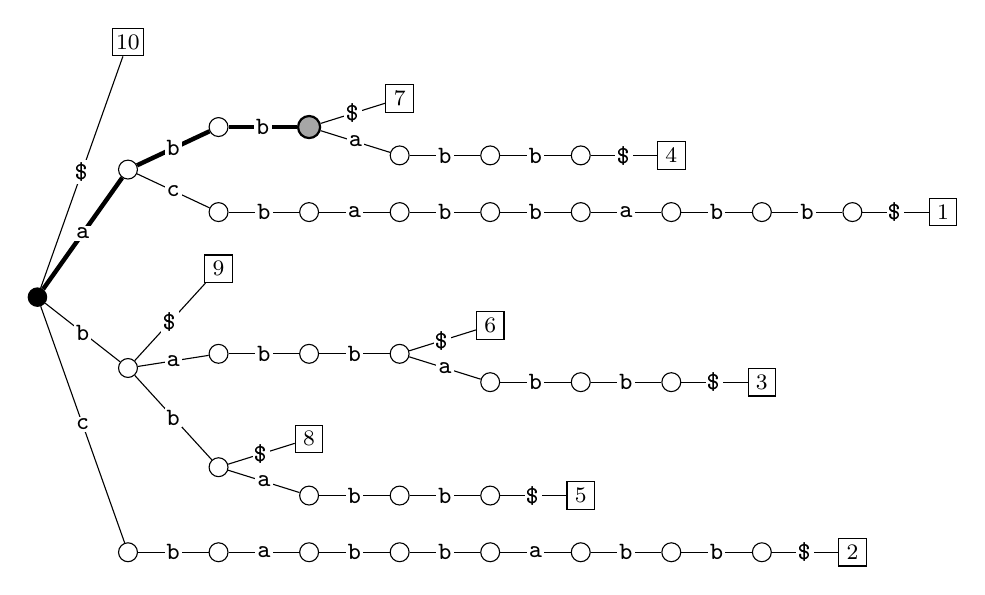
\begin{tikzpicture}[
    trt/.style={circle, draw, thick, fill=black, minimum size=2.2mm, inner sep=0pt},
    tin/.style={circle, draw, minimum size=2.4mm, inner sep=0pt},
    thn/.style={circle, draw, thick, fill=black!35, minimum size=2.8mm, inner sep=0pt},
    tlf/.style={rectangle, draw, font=\footnotesize, inner sep=1.5pt, minimum size=3.5mm},
    tch/.style={fill=white, inner sep=0.8pt, font=\small},
    ted/.style={}, thl/.style={line width=1.6pt}]
\node[tlf] (t1) at (1.15,0.00) {10};
\node[tlf] (t5) at (4.60,-0.72) {7};
\node[tlf] (t9) at (8.05,-1.44) {4};
\node[tin] (t8) at (6.90,-1.44) {};
\node[tin] (t7) at (5.75,-1.44) {};
\node[tin] (t6) at (4.60,-1.44) {};
\node[thn] (t4) at (3.45,-1.08) {};
\node[tin] (t3) at (2.30,-1.08) {};
\node[tlf] (t18) at (11.50,-2.16) {1};
\node[tin] (t17) at (10.35,-2.16) {};
\node[tin] (t16) at (9.20,-2.16) {};
\node[tin] (t15) at (8.05,-2.16) {};
\node[tin] (t14) at (6.90,-2.16) {};
\node[tin] (t13) at (5.75,-2.16) {};
\node[tin] (t12) at (4.60,-2.16) {};
\node[tin] (t11) at (3.45,-2.16) {};
\node[tin] (t10) at (2.30,-2.16) {};
\node[tin] (t2) at (1.15,-1.62) {};
\node[tlf] (t20) at (2.30,-2.88) {9};
\node[tlf] (t24) at (5.75,-3.60) {6};
\node[tlf] (t28) at (9.20,-4.32) {3};
\node[tin] (t27) at (8.05,-4.32) {};
\node[tin] (t26) at (6.90,-4.32) {};
\node[tin] (t25) at (5.75,-4.32) {};
\node[tin] (t23) at (4.60,-3.96) {};
\node[tin] (t22) at (3.45,-3.96) {};
\node[tin] (t21) at (2.30,-3.96) {};
\node[tlf] (t30) at (3.45,-5.04) {8};
\node[tlf] (t34) at (6.90,-5.76) {5};
\node[tin] (t33) at (5.75,-5.76) {};
\node[tin] (t32) at (4.60,-5.76) {};
\node[tin] (t31) at (3.45,-5.76) {};
\node[tin] (t29) at (2.30,-5.40) {};
\node[tin] (t19) at (1.15,-4.14) {};
\node[tlf] (t43) at (10.35,-6.48) {2};
\node[tin] (t42) at (9.20,-6.48) {};
\node[tin] (t41) at (8.05,-6.48) {};
\node[tin] (t40) at (6.90,-6.48) {};
\node[tin] (t39) at (5.75,-6.48) {};
\node[tin] (t38) at (4.60,-6.48) {};
\node[tin] (t37) at (3.45,-6.48) {};
\node[tin] (t36) at (2.30,-6.48) {};
\node[tin] (t35) at (1.15,-6.48) {};
\node[trt] (t0) at (0.00,-3.24) {};
\draw[ted] (t0) -- node[tch] {\texttt{\$}} (t1);
\draw[ted] (t4) -- node[tch] {\texttt{\$}} (t5);
\draw[ted] (t8) -- node[tch] {\texttt{\$}} (t9);
\draw[ted] (t7) -- node[tch] {\texttt{b}} (t8);
\draw[ted] (t6) -- node[tch] {\texttt{b}} (t7);
\draw[ted] (t4) -- node[tch] {\texttt{a}} (t6);
\draw[thl] (t3) -- node[tch] {\texttt{b}} (t4);
\draw[thl] (t2) -- node[tch] {\texttt{b}} (t3);
\draw[ted] (t17) -- node[tch] {\texttt{\$}} (t18);
\draw[ted] (t16) -- node[tch] {\texttt{b}} (t17);
\draw[ted] (t15) -- node[tch] {\texttt{b}} (t16);
\draw[ted] (t14) -- node[tch] {\texttt{a}} (t15);
\draw[ted] (t13) -- node[tch] {\texttt{b}} (t14);
\draw[ted] (t12) -- node[tch] {\texttt{b}} (t13);
\draw[ted] (t11) -- node[tch] {\texttt{a}} (t12);
\draw[ted] (t10) -- node[tch] {\texttt{b}} (t11);
\draw[ted] (t2) -- node[tch] {\texttt{c}} (t10);
\draw[thl] (t0) -- node[tch] {\texttt{a}} (t2);
\draw[ted] (t19) -- node[tch] {\texttt{\$}} (t20);
\draw[ted] (t23) -- node[tch] {\texttt{\$}} (t24);
\draw[ted] (t27) -- node[tch] {\texttt{\$}} (t28);
\draw[ted] (t26) -- node[tch] {\texttt{b}} (t27);
\draw[ted] (t25) -- node[tch] {\texttt{b}} (t26);
\draw[ted] (t23) -- node[tch] {\texttt{a}} (t25);
\draw[ted] (t22) -- node[tch] {\texttt{b}} (t23);
\draw[ted] (t21) -- node[tch] {\texttt{b}} (t22);
\draw[ted] (t19) -- node[tch] {\texttt{a}} (t21);
\draw[ted] (t29) -- node[tch] {\texttt{\$}} (t30);
\draw[ted] (t33) -- node[tch] {\texttt{\$}} (t34);
\draw[ted] (t32) -- node[tch] {\texttt{b}} (t33);
\draw[ted] (t31) -- node[tch] {\texttt{b}} (t32);
\draw[ted] (t29) -- node[tch] {\texttt{a}} (t31);
\draw[ted] (t19) -- node[tch] {\texttt{b}} (t29);
\draw[ted] (t0) -- node[tch] {\texttt{b}} (t19);
\draw[ted] (t42) -- node[tch] {\texttt{\$}} (t43);
\draw[ted] (t41) -- node[tch] {\texttt{b}} (t42);
\draw[ted] (t40) -- node[tch] {\texttt{b}} (t41);
\draw[ted] (t39) -- node[tch] {\texttt{a}} (t40);
\draw[ted] (t38) -- node[tch] {\texttt{b}} (t39);
\draw[ted] (t37) -- node[tch] {\texttt{b}} (t38);
\draw[ted] (t36) -- node[tch] {\texttt{a}} (t37);
\draw[ted] (t35) -- node[tch] {\texttt{b}} (t36);
\draw[ted] (t0) -- node[tch] {\texttt{c}} (t35);
\end{tikzpicture}
\end{center}

\textbf{找 \texttt{abb}}：從根走 \texttt{a}、\texttt{b}、\texttt{b} 三步，走得完，所以 \texttt{abb} 是 $S$ 的子字串。
走到的節點底下有兩個葉節點 $4$ 和 $7$，表示以位置 $4$、$7$ 開始的後綴都以 \texttt{abb} 開頭：
\[
\texttt{acb}\underline{\texttt{abb}}\texttt{abb} \quad\text{和}\quad \texttt{acbabb}\underline{\texttt{abb}},
\]
\texttt{abb} 出現在位置 $4$（$S[4..6]$）和位置 $7$（$S[7..9]$），共兩次。 （下標從 $0$ 算就是位置 $3$ 和 $6$。）
查詢只走了 $|P| = 3$ 步，加上列出底下的葉節點，和 $S$ 的長度無關。

\textbf{大小}：長度 $n$ 的字串，後綴 trie 最多有 $n(n+1)/2 + 1$ 個節點，這裡 $n = 10$（含 \texttt{\$}）時上界是
$56$，實際 $44$ 個。 把只有一個子節點的鏈壓縮起來就是後綴樹，節點數降到 $O(n)$。
\end{pastsoln}
